
\documentclass[10pt,fleqn]{beamer}

\usetheme{Madrid}
\usepackage{xmpmulti}
\usefonttheme[onlylarge]{structurebold}
\setbeamerfont*{frametitle}{size=\normalsize,series=\bfseries}
\setbeamertemplate{navigation symbols}{}

% One color per project
\usecolortheme{DSLAB}
%\usecolortheme{ANAQOE} % descomentar para QoE
%\usecolortheme{ANASECURITY}
% Standard packages


\usepackage[utf8]{inputenc}
\usepackage[T1]{fontenc}
\usepackage[english]{babel}
\usepackage{pgf}
\usepackage{amsmath}
\usepackage{amsfonts}
\usepackage{graphicx}
\usepackage{color}
\usepackage{lmodern}
\usepackage{hyperref}
\usepackage{eurosym}
\usepackage{subfig}
\usepackage{wrapfig}
\usepackage{hyperref} 

% Setup TikZ

\usepackage{tikz}
\usetikzlibrary{arrows}
\tikzstyle{block}=[draw opacity=0.7,line width=1.4cm]


%%%%%%%%%%%%%%%%%%%%%%%%%%%%%%%%%%%%%%%%%%%%%%%%%%%%%%%%%%%%%%%%%%%%%%%%%%%%%%%%
% title page definition %%%%%%%%%%%%%%%%%%%%%%%%%%%%%%%%%%%%%%%%%%%%%%%%%%%%%%%%
%%%%%%%%%%%%%%%%%%%%%%%%%%%%%%%%%%%%%%%%%%%%%%%%%%%%%%%%%%%%%%%%%%%%%%%%%%%%%%%%
\setbeamercovered{dynamic}
\setbeamerfont{author}{family=\rmfamily}
\institute[]{}
\author[Adrián Alonso Barriuso]{Trabajo fin de Máster\\
\vspace{0.5cm}Máster en Ingeniería en Sistemas de Decisión \\ \vspace{1cm}
\scriptsize{Adrián Alonso Barriuso}}
\title[URJC]{Marco de trabajo para evaluar la relevancia de artículos de dominio específico}

\date[Jul 2019]{9 Jul 2019}
%\titlegraphic{
\includegraphics[width=3cm]{DSLab_logo_1.png}}
\def\UrlBreaks{\do\/\do-}
\setbeamertemplate{caption}[numbered]


% The main document

\begin{document}
% transparencia presentación
\begin{frame}
  \titlepage
\end{frame}

\begin{frame}
\frametitle{Index}
\tableofcontents
\end{frame}

\section{Introducción}
\begin{frame}
\begin{figure}
  \centering
  
\includegraphics[width=7cm, keepaspectratio]{images/rese.png}
\end{figure}
  \frametitle{Introducción}
La comunidad investigadora se enfrenta cada vez a un mayor número de publicaciones y tendencias que deben atender a la hora hacer sus propias publicaciones. Estos tópicos y tendencias pueden ser estado del arte en el momento de su publicación en revistas o presentación en conferencias, no obstante, pueden perder relevancia a lo largo del tiempo. Por tanto, la posibilidad de obtener una medida de relevancia de un artículo puede ser de gran utilidad para la comunidad científica.
\end{frame}

\section{Objetivos}
\subsection{Objetivos general}
\begin{frame}\frametitle{Objetivo general} 
El principal objetivo del presente trabajo es la creación de un sistema completo de evaluación
de relevancias, lo que comprende un marco de trabajo que incluye la interfaz para la introducción de documentos y a la salida devuelva la relevancia de los mismos.

\begin{figure}  \centering
  
\includegraphics[width=9cm, keepaspectratio]{relevant-content.jpg}
\end{figure}
\end{frame}

\subsection{Objetivos específicos}
\begin{frame}\frametitle{Objetivos específicos} 
\begin{itemize}
\item Obtención del corpus de documentos científicos. 
\item Limpieza y almacenaje de los documentos.
\item Construcción del lexicón de relevancias.
\item Construcción de la red neuronal.
\item Creación del flujo de evaluación de relevancia.
\end{itemize}
\end{frame}


\section{Propuesta}
\subsection{Arquitectura del sistema}

\begin{frame}\frametitle{Arquitectura básica} 
\begin{figure}
  \centering
  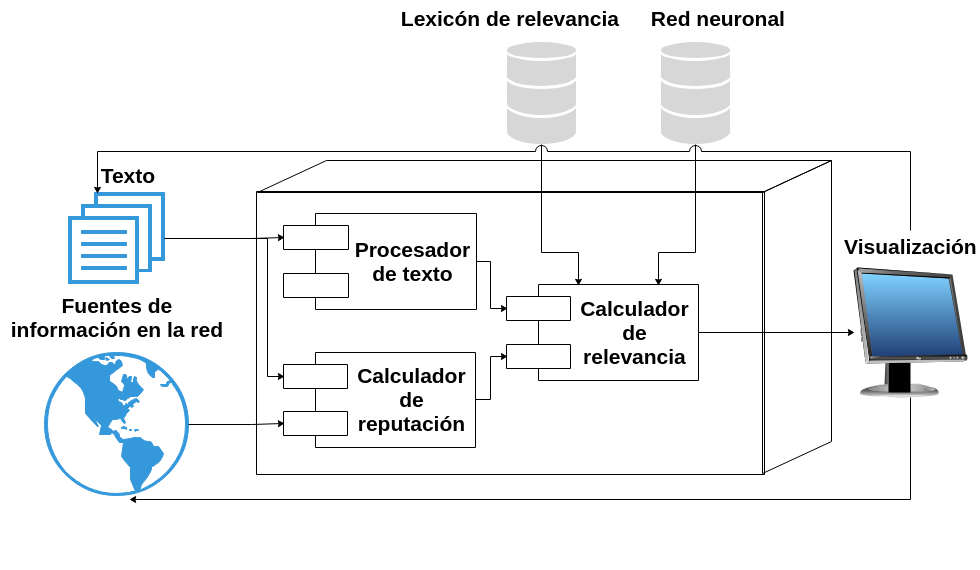
\includegraphics[width=12cm, keepaspectratio]{images/arc_esp.png}
\end{figure}
\end{frame}

\subsection{Recolección y preparación de datos}
\begin{frame} \frametitle{Preparación de los artículos} 
\begin{itemize}
\item Descarga, limpieza y parseo de artículos.
\item Cálculo de resúmenes automáticos.
\item Cálculo de reputaciones.
La reputación de un artículo viene dada por la siguiente fórmula:
\begin{equation}
	rep_{p} = \alpha * 	rep\_authors_{p}  + (1 - \alpha) * citations_{p} \,,
\end{equation}
\begin{equation}\label{eq:1}
	rep\_authors_{p} = \sum  \limits_{i=1}^n  rep_{i} / n \,.
\end{equation}
\begin{equation}
	rep_{i}=\omega_1 * inf\_citation\_count + \omega_2 * citation\_velocity+\omega_3 * seniority + \omega_4 * papers \,,
    \label{eq:author_reputation}
\end{equation}


\end{itemize}

\end{frame}

\begin{frame} \frametitle{Generación de lexicón} 

Relevancia de un término $t$ en un corpus $C$:
\begin{equation}
	rel\_lex_{t} =\log\left(\frac{1}{N} \cdot \sum \limits_{p=1}^N \beta  \cdot tfidf(t)_p + (1-\beta) \cdot rep_p\right), \forall p \in C \,,
\label{eq:4}
\end{equation}

Relevancia acumulada por año:
\begin{equation}
	rel\_lex_{t}(y) = \rho \cdot rel\_lex_{t} + (1-\rho)\cdot rel\_lex_{t}(y-1) \,,
\label{eq:5}
\end{equation}

\end{frame}

\begin{frame} \frametitle{Generación del lexicón} 

\begin{figure}  \centering
  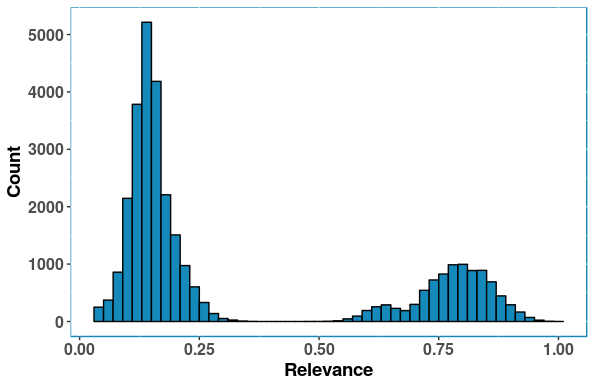
\includegraphics[width=9cm, keepaspectratio]{images/2018_hist.png}
\end{figure}
\end{frame}




\subsection{Creación de la red neuronal}
\begin{frame} \frametitle{Creación de la red neuronal} 
\begin{itemize}
\item Embedding pre-entrenado de 400.000 palabras.
\item Red neuronal convolucional.
\item 320.000 frases train.
\item 80.000 frases test.
\item Salida softmax.
\end{itemize}

\begin{table}[]
\begin{center}
\begin{tabular}{|c|c|}
\hline
\textbf{Año}       & \textbf{Acierto en conjunto de test} \\ \hline
2015      	& $0.964$                \\ \hline
2016        & $0.962$                 \\ \hline
2017 		& $0.959$                 \\ \hline
2018        & $0.959$                  \\ \hline
\end{tabular}
\caption{Resultados de test de las redes neuronales}
\label{tab:red_tests}
\end{center}
\end{table}

\end{frame}


\subsection{Estimación de relevancia}
\begin{frame} \frametitle{Estimación de relevancia de artículos} 

-Relevancia combinada entre lexicón y red neuronal:
\begin{equation}
	combined\_rel_{p} = \theta \cdot rel\_lex_{p} + (1-\theta) \cdot \frac{1}{K} \sum \limits_{k=1}^K rel\_neural(s_k)\,,
    \label{eq:7}
\end{equation}

-Relevancia final combinada con reputación:
\begin{equation}
	combined\_rel\_doi_{p} = \gamma \cdot combined\_rel_{p} + (1-\gamma)\cdot rep_{p} \,,
    \label{eq:8}
\end{equation}

\end{frame}

\begin{frame} \frametitle{Proceso completo} 

\begin{figure}  \centering
  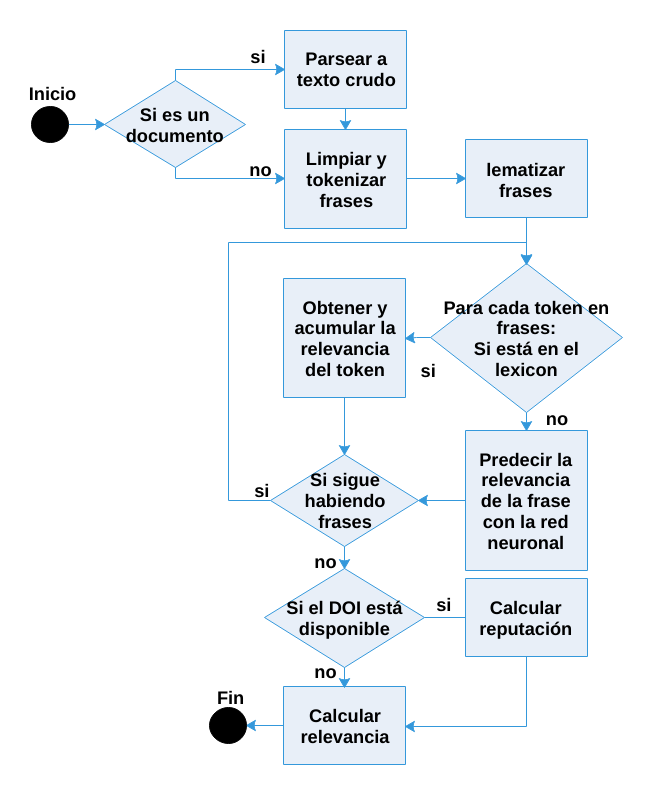
\includegraphics[width=6.5cm, keepaspectratio]{images/pipeline_esp.png}
\end{figure}

\end{frame}


\section{Experimentos}

\begin{frame} \frametitle{Experimentos} 

Resultados 2000 artículos analizados del 2016:
\begin{figure}  \centering
  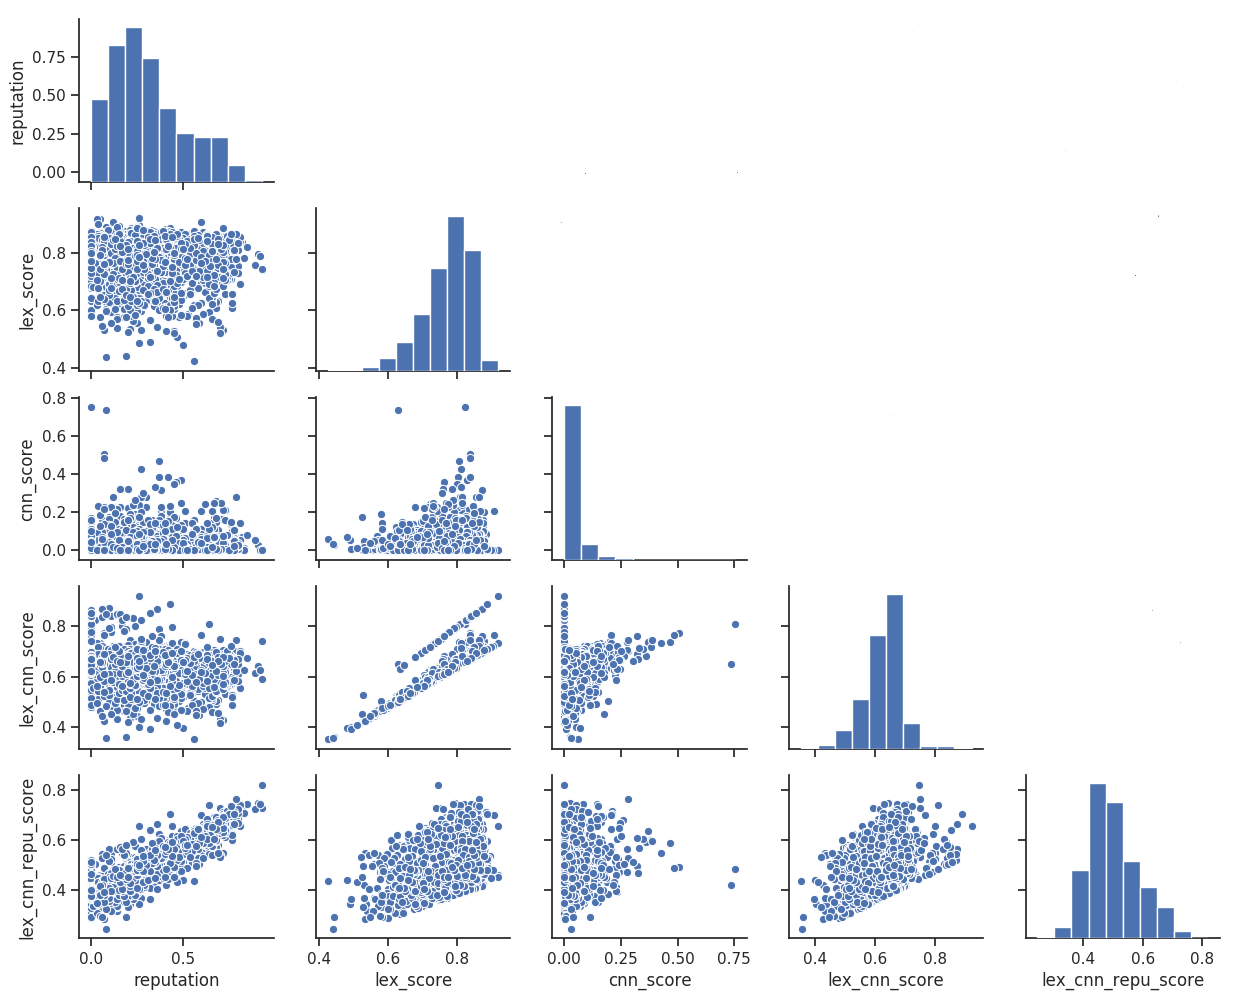
\includegraphics[width=9cm, keepaspectratio]{images/2016_results_mod.png}
\end{figure}

\end{frame}



\begin{frame} \frametitle{Experimentos} 

\begin{figure}  \centering
  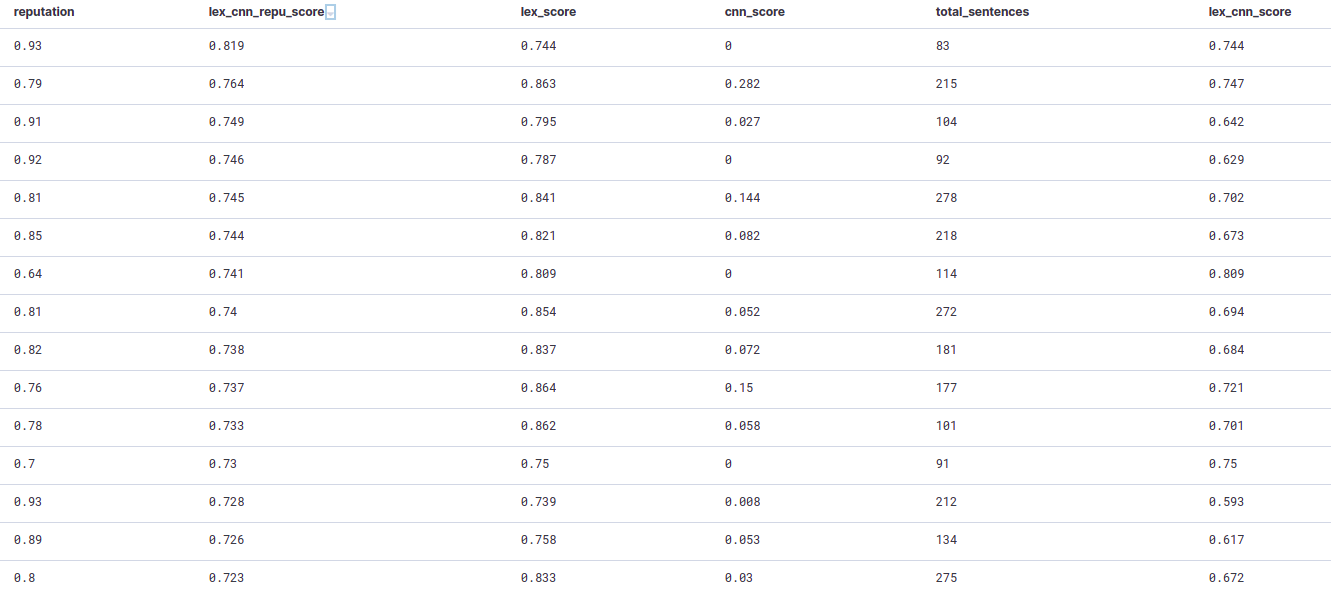
\includegraphics[width=12.5cm, keepaspectratio]{images/kib1.png}
\end{figure}

\end{frame}

\section{Trabajos futuros}
\begin{frame} \frametitle{Trabajos futuros} 
\begin{itemize}
\item Aumento de tamaño de los lexicones.
\item Implementar, probar y comparar otras métricas de relevancia.
\item Detección de correferencias de términos.
\item Creación de word embeddings a partir del corpus.
\item Sustituir sustantivos por conceptos de n-gramas en base a diccionarios u ontologías.

\end{itemize}
\end{frame}

\end{document}